\documentclass[draft=false
              ,paper=a4
              ,twoside=false
              ,fontsize=11pt
              ,headsepline
              ,BCOR=10mm
              ,DIV=11
              ]{scrbook}
\usepackage[ngerman,english]{babel}
%% see http://www.tex.ac.uk/cgi-bin/texfaq2html?label=uselmfonts
\usepackage[T1]{fontenc}
\usepackage[utf8]{inputenc}
\usepackage{libertine}
\usepackage{pifont}
\usepackage{microtype}
\usepackage{textcomp}
\usepackage[german,refpage]{nomencl}
\usepackage{setspace}
\usepackage{makeidx}
\usepackage{listings}
\usepackage{natbib}
\usepackage[ngerman,colorlinks=true]{hyperref}
\usepackage{soul}
\usepackage{hawstyle}
\usepackage{float}
\usepackage{lipsum} %% for sample text

%% define some colors
\colorlet{BackgroundColor}{gray!20}
\colorlet{KeywordColor}{blue}
\colorlet{CommentColor}{black!60}
%% for tables
\colorlet{HeadColor}{gray!60}
\colorlet{Color1}{blue!10}
\colorlet{Color2}{white}

%% configure colors
\HAWifprinter{
  \colorlet{BackgroundColor}{gray!20}
  \colorlet{KeywordColor}{black}
  \colorlet{CommentColor}{gray}
  % for tables
  \colorlet{HeadColor}{gray!60}
  \colorlet{Color1}{gray!40}
  \colorlet{Color2}{white}
}{}
\lstset{%
  numbers=left,
  numberstyle=\tiny,
  stepnumber=1,
  numbersep=5pt,
  basicstyle=\ttfamily\small,
  keywordstyle=\color{KeywordColor}\bfseries,
  identifierstyle=\color{black},
  commentstyle=\color{CommentColor},
  backgroundcolor=\color{BackgroundColor},
  captionpos=b,
  fontadjust=true
}
\lstset{escapeinside={(*@}{@*)}, % used to enter latex code inside listings
        morekeywords={uint32_t, int32_t}
}
\ifpdfoutput{
  \hypersetup{bookmarksopen=false,bookmarksnumbered,linktocpage}
}{}

%% more fancy C++
\DeclareRobustCommand{\cxx}{C\raisebox{0.25ex}{{\scriptsize +\kern-0.25ex +}}}

\clubpenalty=10000
\widowpenalty=10000
\displaywidowpenalty=10000

% unknown hyphenations
\hyphenation{
}

%% recalculate text area
\typearea[current]{last}

\makeindex
\makenomenclature

\begin{document}
\selectlanguage{ngerman}

%%%%%
%% customize (see readme.pdf for supported values)
\HAWThesisProperties{Author={Johanna Böttcher, Marcel Eßmann,\\ Peter Fischer, Jannik Wendt}
                    ,Title={Modulares Keypad}
                    ,EnglishTitle={Developing software in Germany}
                    ,ThesisType={Bussysteme und Sensorik - Projekt}
                    ,ExaminationType={Bachelorprüfung}
                    ,DegreeProgramme={Bachelor of Science Angewandte Informatik}
                    ,ThesisExperts={Prof. Dr. Robert Fitz}
                    ,ReleaseDate={17. Dezember 2024}
                  }

%% title
\frontmatter

%% output title page
\maketitle

\onehalfspacing

%% add abstract pages
%% note: this is one command on multiple lines
%% enable if these lists should be shown on their own page
%%\listoftables
%%\listoffigures
\tableofcontents
\lstlistoflistings

%% main
\mainmatter
\onehalfspacing
%% write to the log/stdout
\typeout{===== File: chapter 1}
%% include chapter file (chapter1.tex)
%%\include{chapter1}


%%%%%%%%%%%%%%%%%%HIER DIE INCLUDES REIN %%%%%%%%%%%%%%%%%%%%%%%%%%%%%%%

%REIHENFOLGE HIER ÄNDERN!
\include{Kapitel/einleitung}
\chapter{Modulares Eingabesystem}
\section{Vision}
Das Eingabesystem verfolgt die Vision eines flexiblen und erweiterbaren Steuerungssystems, das sich an die individuellen Bedürfnisse der Benutzer anpasst. Im Zentrum dieser Vision steht ein Hauptmodul, das als Mikrocontroller-Einheit dient und über eine USB-Schnittstelle mit einem Computer verbunden wird. Dieses Hauptmodul koordiniert die Kommunikation und Funktionalität der angeschlossenen Module.
\\
\\
Die Module des Systems, wie das Tastatur-Modul mit einer 4x4-Tastenmatrix oder das Audio-Modul mit Potentiometern und Fadern, sind frei kombinierbar und können je nach Anwendungsfall hinzugefügt oder entfernt werden. Dies ermöglicht eine maßgeschneiderte Konfiguration für unterschiedliche Aufgaben wie Textverarbeitung, Bildbearbeitung, Audiobearbeitung oder Gaming.
\\
\\
Die folgende Abbildung gewährt einen Überblick über das Eingabesystem:
\begin{figure}[H]
    \centering    
    \fbox{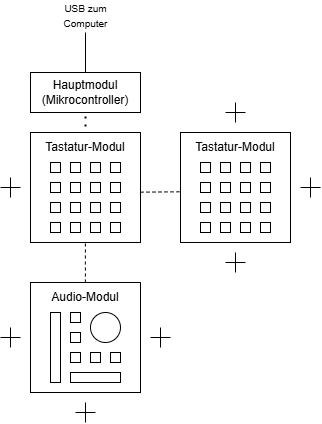
\includegraphics[width=.75\textwidth]{Bilder/bu_vision.png}}
    \caption{Vereinfachte Darstellung des Eingabesystems}
    \label{A3TPHP}
\end{figure}
\noindent Die gestrichelten Linien stellen eine bereits hergestellte Verbindung zwischen den Modulen dar, wobei die \glqq Plus\grqq{} Symbole einen weiteren möglichen Modulanschluss darstellen. Die Module werden untereinander durch die Verwendung von Pogo-Pin-Steckern verbunden.
\subsection{Steckverbindung}
Zwischen den Modulen werden Daten und Spannungsversorgung über eine 4 Pin-Verbindung realisiert. Diese sind VCC (Spannungsversorgung), Data + (Datenbus), Data - (invertierter Datenbus) und GND (Masse). Da der Benutzer die Möglichkeit haben soll, jedes Modul an jede Seite eines anderen anstecken zu können, werden pro Seite zwei 2-Pin Pogo Stecker verwendet, ein 2-Pin Male und ein 2-Pin Female Stecker. Dadurch kann durch kluge Positionierung jede Seite eines Moduls mit jeder Seite eines anderen verbunden werden.
\begin{figure}[H]
    \centering    
    \fbox{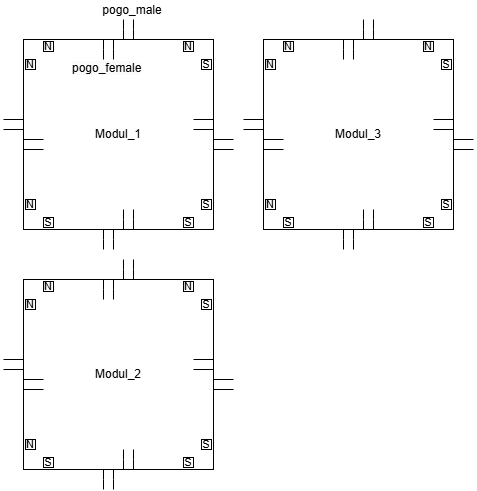
\includegraphics[width=.75\textwidth]{Bilder/bu_pogoverbindung.png}}
    \caption{Pogo verbindung}
    \label{pogo_verbindung}
\end{figure}
 \noindent Abbildung \ref{pogo_verbindung} zeigt, dass die Steckverbindungen eine beliebige Anordnung der Module zulassen.
\chapter{Projektplanung}
\section{}
\subsection{}
\section{Datenbus}
Ein zentraler Bestandteil des modularen Eingabesystems ist das Entwerfen und Umsetzen eines leistungsfähigen und flexiblen Datenbusses. Dieser Datenbus dient als Kommunikationsschnittstelle zwischen den verschiedenen Modulen, wie dem Keypad-Modul und dem Audiomodul und ermöglicht dadurch die Datenübertragung zum Hauptmodul. Skalierbarkeit, Zuverlässigkeit und Geschwindigkeit sind die Hauptkriterien des Datenbusses. Ziel ist es, eine einfache Erweiterbarkeit durch Hinzufügen oder Entfernen von Modulen zu ermöglichen, ohne dabei grundlegende Kommunikationsmechanismen zu beeinträchtigen.

\section{Aufbau des Datenbusses}
Der Bus ist nach folgendem Schema aufgebaut:
\begin{itemize}
    \item Start of Frame (SOF) - 2 Bit zum Synchronisieren der Frequenzen
    \item Sendeadresse -  3 Bit zum Senden der Adresse
    \item ?? (COF) - 3 Bit für Datenlänge in Byte
    \item Daten - X Byte
    \item ?? (CRC) - X Bit
    \item Enf of Frame (EOF) - 4 Bit LOW, Signalende
\end{itemize}

Die folgende Abbildung stellt den Datenbus dar:
\begin{figure}[H]
    \centering    
    \includegraphics[width=1\textwidth]{}
    \caption{Aufbau des Datenbusses}
    \label{Datenbus}
\end{figure}

\section{Aktueller Stand}
\subsection{}
\section{Programme}
Für die Module gibt es ein Programcode, wo mithilfe von #define definiert wird um welche Art von Modul es sich handelt. Je nach Modultyp werden nur gewisse Funktionen genutzt:
% hier tabelle einfügen


Wir haben uns für diese Herangehensweise entschieden, da bei der Programmierung größere Mengen von Microkontrollern falsche Software geflashed werden könnte wenn es mehrere sehr ähnlich aussehende Programme gibt. Zusätzlich ist die Entwicklung neuer Funktionen deutlich einfacher, da eine für alle Module notwendige Änderung nicht in mehrere Quelldateien angepasst werden muss.


\subsection{Hauptmodul}


\subsection{Tastaturmodul}
\subsection{Übersetzerprogramm}
Um die HEX-Werte aus der UART Verbindung vom Hauptmodul am Computer auszuwerten wird ein Python Script geschrieben, welches diese einließt und auswertet. Mit unserem aktuellen Prototypen lassen sich so die vier Tasten beliebig "belegen" und zum Beispiel eine Powerpoint Präsentation steuern.
\\

\section{Modulübergreifende Funktionen}
\textmd{Die Funktionen zum Lesen und Senden von Nachrichten müssen auf allen Modulen implementiert werden.\\
}
\subsection{Senden einer Nachricht}
\textmd{Um eine Nachricht auf den Bus zu schreiben, muss zunächst festgestellt werden, dass dieser gerade nicht beschrieben wird.\\
	Nur wenn dies der Fall ist, kann die Nachricht gesendet werden. \\
	Die Nachricht setzt sich aus den in Kapitel \ref{} beschriebenen Teilen zusammen. Jedes dieser Teile wurde als eigenen Funktion implementiert und schlussendlich in einer übergreifenden Funktion zusammengeführt.\\
}

\lstinputlisting[firstline= 10, lastline=20,language = C++,frame=single,label=send(),caption=Senden einer Nachricht]{
	Programme/main.cpp}



\subsection{Empfangen einer Nachricht}
\textmd{Solange ein Modul keine Nachricht versenden möchte hört dieses auf die Nachrichten auf dem Bus. Bei jedem Empfang eines Start of Frame wird die Busfrequenz berechnet und gespeichert. Wenn dann die Empfangene Adresse die eigene Adresse ist wird auf den Rest der Nachricht gehört und gespeichert, um diese zu verarbeiten.\\
	Auch hier wurde jeder Teil der Nachricht als eigene Funktion implementiert und in einer übergreifenden Funktion zusammengeführt.
}
\lstinputlisting[firstline= 10, lastline=20,language = C++,frame=single,label=recieve(),caption=Empfangen einer Nachricht]{
	Programme/main.cpp}





\section{Code des Hauptmoduls}
\textmd{Im Folgendem wird der Programm-Ablauf des Hauptmoduls näher beschrieben.\\ 
	Das Hauptmodul übernimmt folgende Aufgaben:\\\\
	1. Verwaltung der Adressvergabe an angeschlossene Module\\
	2. Abfrage nach neuen Daten der einzelnen Module\\
	3. Übermittlung dieser Daten über eine UART-Schnittstelle an den angeschlossenen Rechner\\\\ 
}
\begin{figure}[H]
	\centering    
	\includegraphics[width=.75\textwidth]{}
	\caption{Programmablauf Hauptmodul}
	\label{Programm_Hauptmodul}
\end{figure}
\textmd{
}
\subsection{Adressvergabe und Verwaltung}
\textmd{Das Hauptmodul speichert alle vergebenen Adressen zusammen mit der Funktion und einigen weiteren Variablen des jeweiligen Moduls in einer Liste von stucts.\\
	Diese Liste wird zum Polling der Teilnehmer genutzt, sodass nur angeschlossene Module abgefragt werden.\\}


\lstinputlisting[firstline= 10, lastline=20,language = C++,frame=single,label=decice,caption=Struct device]{
	Programme/main.cpp}


\textmd{Die jeweiligen Module haben keine festgelegte Adresse. Wenn diese also mit Spannung versorgt werden warten Sie auf die Adressvergabe des Hauptmoduls.\\
	In der Polling Liste wird eine bestimmte Adresse abgefragt um festzustellen, wenn ein neuer Teilnehmer an den Bus angeschlossen wurde. Wenn eine Rückmeldung auf diese Adresse festgestellt wird, dann enthält die nächste Nachricht die Adresse für den neuen Teilnehmer.
	In der Rückmeldung eines Moduls ist dessen Funktion hinterlegt. Diese Informationen werden in der Adressliste abgespeichert und das Gerät ab dem Zeitpunkt mit abgefragt.\\
}

\newpage
\lstinputlisting[firstline= 10, lastline=20,language = C++,frame=single,label=recieve(),caption=Empfangen einer Nachricht]{Programme/main.cpp}

\textmd{Wenn ein Modul nicht mehr über den Bus kommuniziert wird nach ein paar Versuchen die Adresse wieder aus der Polling Liste herausgeworfen und den verfügbaren Adressen zugewiesen. Somit kann sichergestellt werden, dass alle angeschlossenen Geräte so schnell wie möglich vom Hauptmodul abgefragt werden und zudem auch wieder Adressen für neue Geräte freigemacht.
}

\lstinputlisting[firstline= 10, lastline=20,language = C++,frame=single,label=timeout(),caption=Timeout Funktion]{Programme/main.cpp}

\textmd{Wenn keine Antwort des Slavemoduls in der vorgegebenen Wartezeit empfangen wird, wird der Timeout-Counter iteriert. Sobald dieser seinen Maximalwert erreicht wird das Gerät nicht mehr abgefragt und dessen Adresse freigegeben.
}

\newpage
\subsection{Abfrage neuer Daten}
\textmd{Die Daten eines jeden Moduls werden einmal pro Durchlauf der Polling Liste abgefragt. Wenn neue Daten empfangen wurden werden diese abgespeichert und dem angeschlossenen Computer über die UART-Schnittstelle übermittelt.
}

\lstinputlisting[firstline= 10, lastline=20,language = C++,frame=single,label=polling(),caption=polling]{
	Programme/main.cpp}

\newpage
\subsection{Übermittlung der Daten an den angeschlossenen Computer}
\textmd{Sobald neue Daten von einem Modul empfangen worden sind, werden diese an den Computer übermittelt. Diese Kommunikation erfolgt über eine UART Schnittstelle und den auf dem PCB verbauten UART zu USB Bridge IC. \\
	Zu den übermittelten Daten wird neben der jeweiligen Funktion auch die zugehörige Adresse übermittelt, sodass die Daten nicht nur Abhängig von der Funktion ausgewertet werden können, sondern auch mehrere gleiche Module voneinander unterschieden werden können.  
}
\lstinputlisting[firstline= 10, lastline=20,language = C++,frame=single,label=usb(),caption=Übertragung an den angeschlossenen Computer]{
	Programme/main.cpp}

\section{Code der Slaves}
\textmd{Im Folgendem wird der Programm-Ablauf eines Slaves genauer beschrieben. Die Aufgaben eines Slave-Moduls sind folgende:\\\\
	1. Anfordeung einer Adresse bei Neustart\\
	2. Auswerten der Modulfunktion\\
	3. Übermitteln der Daten an das Hauptmodul bei Anfrage\\
}
\begin{figure}[H]
	\centering    
	\includegraphics[width=.75\textwidth]{}
	\caption{Programmablauf eines Slave-Moduls}
	\label{Programm_Slaves}
\end{figure}
\subsection{Anforderung einer Adresse}
\textmd{Wenn dem Modul noch keine Adresse zugewiesen wurde und der Hauptcontroller nach neuen Teilnehmern auf dem Bus fragt, dann meldet sich dieses Modul mit einer Nachricht, in der die Funktion des Moduls in den Daten übermittelt wird.\\
	Im Anschluss wird der Hauptcontroller die neue Adresse übermitteln. Diese wird von dem Modul gespeichert und es meldet sich dann nur noch auf diese Adresse.
}
\lstinputlisting[firstline= 10, lastline=20,language = C++,frame=single,label=usb(),caption=Anfordern einer Adresse]{
	Programme/main.cpp}

\newpage
\subsection{Auswertung der Modulfunktion}
\textmd{Die Auswertung der Modulfunktion ist abhängig von der jeweiligen Funktion des Moduls und kann aufgrund dessen nicht übergreifend relativiert werden.\\
	Bei dem Tastaturmodul werden die Tasten ausgewertet, sobald der Hauptcontroller das Modul abfragt und im Anschluss übermittelt. Hierzu wurde eine allgemeine Funktion kreiert, die für jedes Modul angepasst werden muss.
}

\lstinputlisting[firstline= 10, lastline=20,language = C++,frame=single,label=myfunction(),caption=Individuelle Funktion]{
	Programme/main.cpp}

\subsection{Übermittlung der Daten an das Hauptmodul}
\textmd{Sobald eine Anfrage des Hauptmoduls an die Adresse des Moduls empfangen wird, übermittelt dieses die Information der Modulfunktion. Im Falle der Tastatur währen dies die zurzeit gedrückten Tasten.
}



\lstinputlisting[language=c++, caption={main.cpp}, label={main.cpp}]{Kapitel/Programme/main.cpp}
\lstinputlisting[language=python, caption={pyscript}, label={pyscript}]{Kapitel/Programme/uart.py}


\section{Fazit}
Die agile Herangehensweise stellt  Herausforderungen dar, insbesondere wenn bisher wenig praktische Erfahrung mit dieser Art der Projektleitung vorhanden ist. Dennoch konnten klare Vorteile der agilen Entwicklung festgestellt werden. So wurde beispielsweise das anfängliche Ziel, mehrere Module zu entwickeln, rechtzeitig angepasst, um den zeitlichen Einschränkungen gerecht zu werden. Darüber hinaus war es möglich, Aufgaben gemeinsam zu bearbeiten oder neu zuzuweisen, wenn einzelne Gruppenmitglieder ausfielen.

Es zeigt sich jedoch, dass eine gründlichere Planungsphase dazu hätte beitragen können, einige Probleme frühzeitig zu erkennen und zu vermeiden. So haben beispielsweise die differenzielle Datenübertragung und das Flashen der ATtinys und ATmegas viel Zeit in Anspruch genommen. Schwierigkeiten, die vermutlich durch eine bessere Abstimmung der Komponenten im Vorfeld hätten reduziert oder ganz vermieden werden können.

Des Weiteren wird in Anbetracht der noch verbleibenden Zeit das Audio-Modul aus dem Plan für dieses Projekt gestrichen und sich erstmal lediglich auf das Tastaturmodul fokussiert. Da dieses Projekt nach Abschluss des Faches \glqq Bussysteme und Sensorik\grqq{} für den privaten Gebrauch der Gruppenmitglieder weiterentwickelt wird, wird dieses Modul wahrscheinlich in Zukunft eingeführt. Das grobe Layout eines weiteren Moduls wird sich nicht grundlegend von dem des Tastaturmoduls unterscheiden, daher liegt die Priorität erstmal in der Optimierung des vorhandenen Moduls.



%%%%

%% appendix if used
%%\appendix
%%\typeout{===== File: appendix}
%%\include{appendix}

% bibliography and other stuff
\backmatter

\typeout{===== Section: literature}
%% read the documentation for customizing the style
\bibliographystyle{dinat}
%\bibliography{sample}
\typeout{===== Section: nomenclature}
\end{document}
